The touchscreen device will retrieve application data from the web server to display information from the current brew.  The display will also offer a Graphical User interface where the user can input commands to modify the current brew. The client application running on this device will then interpret the data, and either display it on the Data Display or send it back to the server as commands accordingly.

\subsection{Data Display}
The data display will display real-time information relevant to the current brew. The data display will retrieve this data from the web server.

\begin{figure}[h!]
	\centering
 	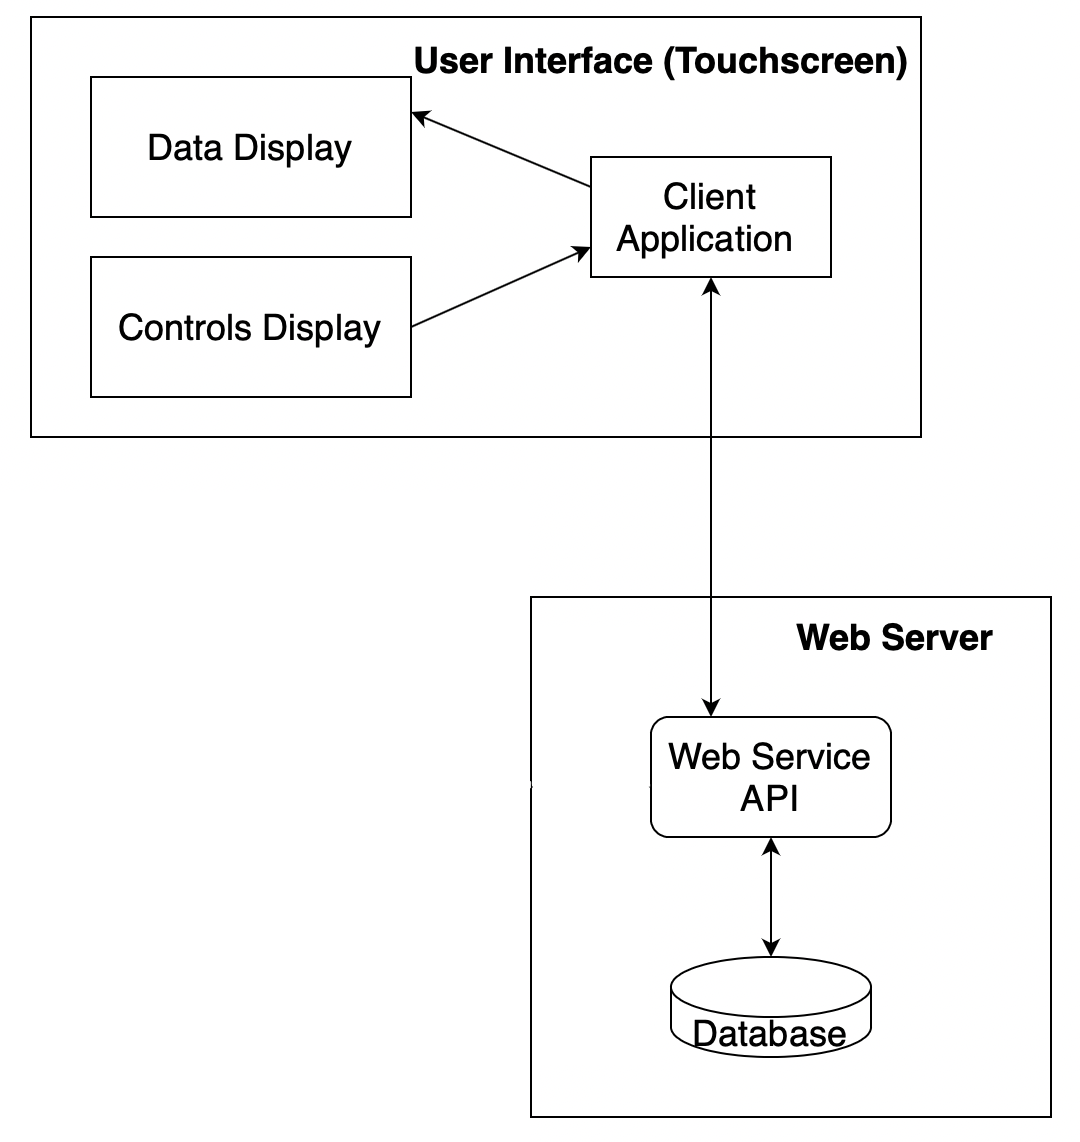
\includegraphics[width=0.60\textwidth]{images/UI_subsystem}
 \caption{User Interface subsystem diagram}
\end{figure}

\subsubsection{Assumptions}
\begin {itemize}
\item The device will receive the data and interpret it correctly on the touchscreen.
\item The data received from the server will be accurate and up-to-date.
\item The device will have a stable connection to the server throughout the brew.
\end {itemize}


\subsubsection{Responsibilities}
The device will receive accurate and relevant information from the server and display it on the touchscreen for the user to make decisions on the current brew. This information will include current set temperature, length of time the temperature has been set, how much longer brew will stay at current temperature, and any other information that may be relevant.

\subsubsection{Subsystem Interfaces}

\begin {table}[H]
\caption {Subsystem interfaces} 
\begin{center}
    \begin{tabular}{ | p{6cm} | p{3cm} | p{3cm} |}
    \hline
    Description & Inputs & Outputs \\ \hline
    Data Display & \pbox{3cm}{Data from \\ server} & \pbox{3cm}{Brew information}  \\ \hline
    \end{tabular}
\end{center}
\end{table}

\subsection{Controls Display}
The controls display on the touchscreen will allow the user to interact with and send commands to the server, which will relay the data to the brewing system.

\begin{figure}[h!]
	\centering
 	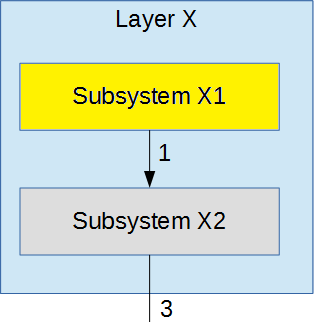
\includegraphics[width=0.60\textwidth]{images/subsystem}
 \caption{Example subsystem description diagram}
\end{figure}

\subsubsection{Assumptions}
\begin {itemize}
\item The client application will read user commands correctly and send them following the established protocol.
\item The device will be quick in sending commands to the server.
\item The device will have a stable connection to the server throughout the brew.
\end {itemize}


\subsubsection{Responsibilities}
The touchscreen will allow the user to enter commands such as set, increase, or decrease temperature and/or the length of time temperature is set. The interface will be intuitive and easy to use. The client application will then take the commands, and send them to the server following the set communcation protocol. Commands sent will update the information on the data display if applicable.

\subsubsection{Subsystem Interfaces}

\begin {table}[H]
\caption {Subsystem interfaces} 
\begin{center}
    \begin{tabular}{| p{6cm} | p{3cm} | p{3cm} |}
    \hline
    Description & Inputs & Outputs \\ \hline
    Controls Display & \pbox{3cm}{User input} & \pbox{3cm}{Data to \\ server}  \\ \hline
    \end{tabular}
\end{center}
\end{table}


